% Source : http://tex.stackexchange.com/questions/38032/create-an-array-in-tikz-with-underbrace-in-different-colors

\documentclass{article}
	\usepackage{tikz}
	\usetikzlibrary{decorations.pathreplacing,shapes}


\begin{document}

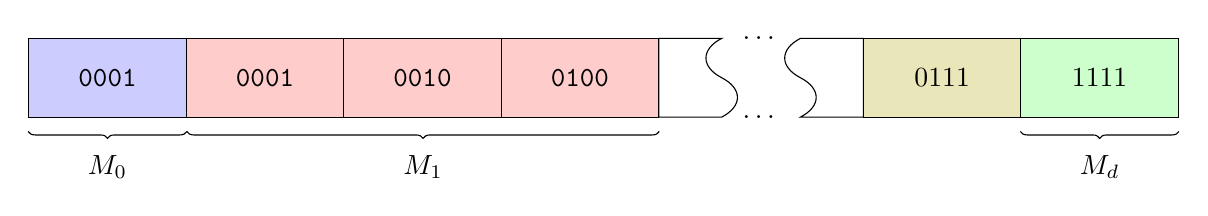
\begin{tikzpicture}
	\foreach \c/\i [count=\n] in {
		blue!20/0001,
		red!20/0001,
		red!20/0010,
		red!20/0100
	}
		\node[
			draw,
			fill=\c,
			minimum height=1cm,
			minimum width = 2cm,
			xshift=\n*2cm,
			font=\ttfamily
		](N\n){\i} ;

	\draw[
		decoration={brace,mirror,raise=5pt},
		decorate
	] (N1.south west) --  node[below=10pt]{$M_0$}(N1.south east);

	\draw[
		decoration={brace,mirror,raise=5pt},
		decorate
	] (N1.south east) --  node[below=10pt]{$M_1$}(N4.south east);

	\node[
		tape,
		draw,
		minimum size=1cm,
		tape bend top=none,
		tape bend height=0.4cm,
		rotate=90
	] at (9.3,0) (t) {};

	\node[
		tape,
		draw,
		minimum size=1cm,
		tape bend top=none,
		tape bend height=0.4cm,
		rotate=270
	] at (11.3,0) (t) {};

	\node at (10.3,0.5) {\dots};
	\node at (10.3,-0.5) {\dots};

	\foreach \c/\i [count=\m] in {
		olive!20/0111,
		green!20/1111
	}
		\node[
			draw,
			fill=\c,
			minimum height=1cm,
			minimum width = 2cm,
			xshift=10.6cm+\m*2cm
		] (N\m) {\i} ;

	\draw [
		decoration={brace,mirror,raise=5pt},
		decorate
	] (N2.south west) -- node[below=10pt]{$M_d$}(N2.south east);
\end{tikzpicture}

\end{document}
